%META {"question":"Ot và Ou lần lượt là tia phân giác của hai góc kề bù xOz và zOy. Góc tOu bằng bao nhiêu?","options":["90°","45°","180°","60°"],"answer":0,"note":"Góc tOu = một nửa góc xOz cộng một nửa góc zOy, tức bằng một nửa góc bẹt xOy: 180° : 2 = 90°. Hai tia phân giác của hai góc kề bù luôn vuông góc với nhau."}
\documentclass[border=5pt]{standalone}
\usepackage{tkz-euclide}
% Màu dùng chung cho toàn bộ hình vẽ (ảnh stack với nền tối của web)
\definecolor{tminc}{RGB}{226,232,240}   % chữ + nét chính
\definecolor{tmblue}{RGB}{0,210,255}    % nhấn neon xanh
\definecolor{tmpink}{RGB}{255,0,200}    % nhấn neon hồng
\definecolor{tmgreen}{RGB}{0,255,136}   % nhấn neon xanh lá
\color{tminc}

\begin{document}
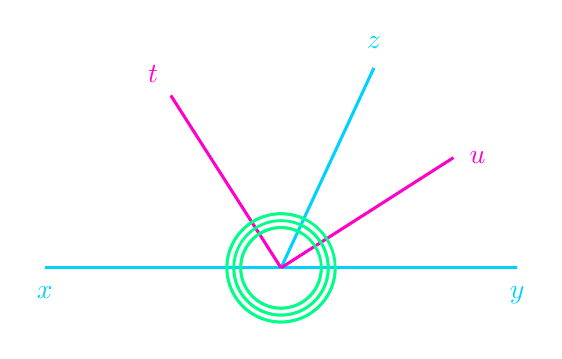
\begin{tikzpicture}[line width=1.1pt]
  \coordinate (O) at (0,0);
  \coordinate (X) at (-3,0);
  \coordinate (Y) at (3,0);
  \coordinate (Z) at (1.18,2.54);
  \coordinate (T) at (-1.4,2.19);
  \coordinate (U) at (2.19,1.4);
  \draw[tmblue] (O) -- (X) node[below=3pt]{$x$};
  \draw[tmblue] (O) -- (Y) node[below=3pt]{$y$};
  \draw[tmblue] (O) -- (Z) node[above=3pt]{$z$};
  \draw[tmpink] (O) -- (T) node[above left=1pt]{$t$};
  \draw[tmpink] (O) -- (U) node[right=2pt]{$u$};
  \tkzMarkAngles[size=0.6,arc=l,color=tmgreen,line width=1pt](X,O,T)
  \tkzMarkAngles[size=0.6,arc=l,color=tmgreen,line width=1pt](T,O,Z)
  \tkzMarkAngles[size=0.6,arc=ll,color=tmgreen,line width=1pt](Z,O,U)
  \tkzMarkAngles[size=0.6,arc=ll,color=tmgreen,line width=1pt](U,O,Y)
\end{tikzpicture}
\end{document}
